\documentclass[12pt,letterpaper]{article}
\usepackage[T1]{fontenc}
\usepackage{helvet}
\renewcommand{\familydefault}{\sfdefault}
\usepackage[letterpaper,left=0.58in,right=0.58in,top=0.72in,bottom=0.62in,headheight=15pt,headsep=13pt,footskip=22pt]{geometry}
\usepackage{tikz}
\usepackage{fancyhdr}
\usetikzlibrary{arrows.meta,calc}
\setlength{\parindent}{0pt}
\setlength{\parskip}{6pt}
\pagestyle{fancy}
\fancyhf{}
\renewcommand{\headrulewidth}{0.3pt}
\renewcommand{\footrulewidth}{0pt}
\fancyfoot[L]{\footnotesize Bellingham Math Circle / Week 12 / W12-RV-v1}
\fancyfoot[R]{\footnotesize\thepage}
\newcommand{\pagehead}[1]{\fancyhead[L]{\small Week 12 / Pairings and paths / #1}}
\newcommand{\problem}[2]{\textbf{Problem #1:} #2\par}
\definecolor{redcounter}{RGB}{173,44,54}
\definecolor{bluecounter}{RGB}{31,99,165}

% Large boards are 3 inches in diameter; all circles use the same six places.
\newcommand{\pairboard}[3]{%
  \begin{tikzpicture}[x=#1in,y=#1in,baseline=(current bounding box.center)]
  \path[use as bounding box] (-1.13,-1.11) rectangle (1.13,1.13);
  \node[font=\bfseries\small] at (-1,1.02) {#3};
  \draw[gray!65,line width=.65pt] (0,0) circle (1);
  \foreach \letter [count=\i] in {#2} {
    \pgfmathsetmacro{\ang}{90-(\i-1)*60}
    \ifx\letter\empty\else
      \if\letter R
        \node[circle,draw=redcounter,fill=redcounter!12,minimum size=19pt,inner sep=0pt,font=\bfseries\small] at (\ang:1) {R};
      \else
        \node[circle,draw=bluecounter,fill=bluecounter!12,minimum size=19pt,inner sep=0pt,font=\bfseries\small] at (\ang:1) {B};
      \fi
    \fi
  }
  \end{tikzpicture}%
}
% Full labels and the same case marker keep each saved pairing recoverable.
\newcommand{\recordpair}[2]{%
  \begin{tikzpicture}[x=.55in,y=.55in,baseline=(current bounding box.center)]
  \path[use as bounding box] (-1.2,-1.2) rectangle (1.2,1.2);
  \node[font=\bfseries\small] at (-1,1.02) {#2};
  \draw[gray!60,line width=.45pt] (0,0) circle (1);
  \foreach \letter [count=\i] in {#1} {
    \pgfmathsetmacro{\ang}{90-(\i-1)*60}
    \if\letter R
      \node[circle,draw=redcounter,fill=redcounter!12,minimum size=11pt,inner sep=0pt,font=\bfseries\scriptsize] at (\ang:1) {R};
    \else
      \node[circle,draw=bluecounter,fill=bluecounter!12,minimum size=11pt,inner sep=0pt,font=\bfseries\scriptsize] at (\ang:1) {B};
    \fi
  }
  \end{tikzpicture}%
}
\newcommand{\recordgroup}[2]{%
  \begin{tabular}{@{}c@{\hspace{.55in}}c@{\hspace{.55in}}c@{}}
  \recordpair{#1}{#2} & \recordpair{#1}{#2} & \recordpair{#1}{#2}\\[3pt]
  \recordpair{#1}{#2} & \recordpair{#1}{#2} & \recordpair{#1}{#2}
  \end{tabular}%
}

% A square unit is the same horizontal and vertical size throughout.
\newcommand{\emptywalk}[2]{%
  \begin{tikzpicture}[x=.86cm,y=.86cm]
  \path[use as bounding box] (-.48,-.38) rectangle (#1+.35,#2+.38);
  \draw[step=1,gray!30,line width=.35pt] (0,0) grid (#1,#2);
  \draw[line width=.9pt] (0,0)--(#1,0);
  \draw[densely dashed,line width=.9pt] (0,#2)--(#1,#2);
  \foreach \h in {0,...,#2} {\node[left,font=\scriptsize] at (0,\h) {\h};}
  \fill (0,0) circle (1.9pt); \fill (#1,0) circle (1.9pt);
  \node[below,font=\scriptsize] at (0,0) {S};
  \node[below,font=\scriptsize] at (#1,0) {E};
  \end{tikzpicture}%
}
\newcommand{\walk}[4]{%
  \begin{tikzpicture}[x=#4cm,y=#4cm,baseline=(current bounding box.center)]
  \path[use as bounding box] (-.5,-.48) rectangle (#1+.2,#2+.45);
  \draw[step=1,gray!30,line width=.35pt] (0,0) grid (#1,#2);
  \draw[line width=.9pt] (0,0)--(#1,0);
  \node[left,font=\scriptsize] at (0,0) {0};
  \draw[line width=1.2pt] plot coordinates {#3};
  \end{tikzpicture}%
}
\newcommand{\routearea}[1]{%
  \begin{tikzpicture}[baseline=(current bounding box.center)]
  \path[use as bounding box] (0,0) rectangle (8.7,#1);
  \draw[gray!40,line width=.4pt] (0,0) rectangle (8.7,#1);
  \end{tikzpicture}%
}

\begin{document}
\pagehead{Grades K--3}
Join each R to a B, using every dot once. Lines must stay inside the circle and must not cross. The dots keep their places.

\problem{1}{Find every pairing for each arrangement.}
\vspace{1pt}
\begin{center}
\begin{tabular}{@{}c@{\hspace{.31in}}c@{}}
\pairboard{1.5}{R,B,R,B,R,B}{A} & \pairboard{1.5}{R,R,R,B,B,B}{B}\\[9pt]
\multicolumn{2}{c}{\pairboard{1.5}{R,R,B,R,B,B}{C}}
\end{tabular}
\end{center}

\newpage
\pagehead{Grades K--3}
Extra workspace
\begin{center}
\recordgroup{R,B,R,B,R,B}{A}\\[7pt]
\recordgroup{R,R,R,B,B,B}{B}\\[7pt]
\recordgroup{R,R,B,R,B,B}{C}
\end{center}

\newpage
\pagehead{Grades 2--5}
U is one diagonal step up and right. D is one diagonal step down and right. A path starts at S and ends at E; it stays on or above 0.

\problem{2}{Use four U steps and four D steps. Find every path that stays at or below the dashed ceiling at height 2.}
\begin{center}
\setlength{\tabcolsep}{4pt}
\begin{tabular}{@{}c@{\hspace{.32in}}c@{}}
\emptywalk{8}{2} & \emptywalk{8}{2}\\[8pt]
\emptywalk{8}{2} & \emptywalk{8}{2}\\[8pt]
\emptywalk{8}{2} & \emptywalk{8}{2}\\[8pt]
\emptywalk{8}{2} & \emptywalk{8}{2}\\[8pt]
\emptywalk{8}{2} & \emptywalk{8}{2}
\end{tabular}
\end{center}
\vspace{5pt}
\problem{3}{With the same ceiling, how many paths use five U steps and five D steps? Find a way to know without drawing every path.}
\vspace{4pt}
\begin{center}
\begin{tikzpicture}
\path[use as bounding box] (0,0) rectangle (16.7,2.2);
\draw[gray!40,line width=.4pt] (0,0) rectangle (16.7,2.2);
\end{tikzpicture}
\end{center}

\newpage
\pagehead{Grades 4--5}
A move swaps neighboring U and D cards. Stay on or above 0 after every move.
\vspace{2pt}
\begin{center}
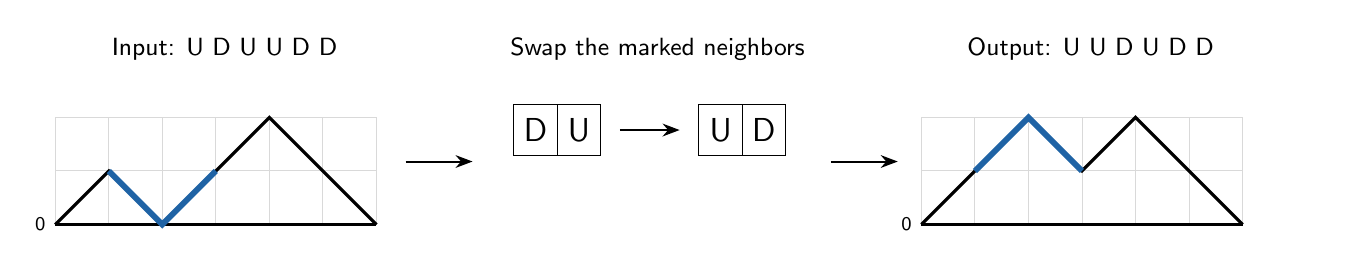
\begin{tikzpicture}[x=1cm,y=1cm,>=Stealth]
\path[use as bounding box] (0,0) rectangle (16.7,2.85);
\node at (2.5,2.58) {\small Input: U D U U D D};
\begin{scope}[shift={(.35,.35)},x=.68cm,y=.68cm]
\draw[step=1,gray!30,line width=.35pt] (0,0) grid (6,2);
\draw[line width=.8pt] (0,0)--(6,0);
\node[left,font=\scriptsize] at (0,0) {0};
\draw[line width=1.15pt] plot coordinates {(0,0)(1,1)(2,0)(3,1)(4,2)(5,1)(6,0)};
\draw[line width=2.1pt,bluecounter] (1,1)--(2,0)--(3,1);
\end{scope}
\draw[->,line width=.7pt] (4.8,1.15)--(5.65,1.15);
\node at (8.0,2.58) {\small Swap the marked neighbors};
\node[draw,minimum width=.55cm,minimum height=.65cm,font=\large] at (6.45,1.55) {D};
\node[draw,minimum width=.55cm,minimum height=.65cm,font=\large] at (7.0,1.55) {U};
\draw[->,line width=.7pt] (7.52,1.55)--(8.28,1.55);
\node[draw,minimum width=.55cm,minimum height=.65cm,font=\large] at (8.8,1.55) {U};
\node[draw,minimum width=.55cm,minimum height=.65cm,font=\large] at (9.35,1.55) {D};
\draw[->,line width=.7pt] (10.2,1.15)--(11.05,1.15);
\node at (13.5,2.58) {\small Output: U U D U D D};
\begin{scope}[shift={(11.35,.35)},x=.68cm,y=.68cm]
\draw[step=1,gray!30,line width=.35pt] (0,0) grid (6,2);
\draw[line width=.8pt] (0,0)--(6,0);
\node[left,font=\scriptsize] at (0,0) {0};
\draw[line width=1.15pt] plot coordinates {(0,0)(1,1)(2,2)(3,1)(4,2)(5,1)(6,0)};
\draw[line width=2.1pt,bluecounter] (1,1)--(2,2)--(3,1);
\end{scope}
\end{tikzpicture}
\end{center}

\problem{4}{Show a shortest route from each start to the target. Can you tell how many moves a path needs before making any moves?}
\begin{center}
\begin{tabular}{@{}c@{\hspace{.3in}}c@{}}
\walk{8}{4}{(0,0)(1,1)(2,2)(3,3)(4,4)(5,3)(6,2)(7,1)(8,0)}{.60} &
\begin{minipage}{3.6in}\centering Target: U U U U D D D D\end{minipage}
\end{tabular}
\end{center}
\vspace{-3pt}
\begin{center}
\begin{tabular}{@{}c@{\hspace{.2in}}c@{}}
\begin{minipage}{2.85in}\centering
\small Start: U D U D U D U D\par
\walk{8}{4}{(0,0)(1,1)(2,0)(3,1)(4,0)(5,1)(6,0)(7,1)(8,0)}{.63}
\end{minipage} & \routearea{5.0}\\[8pt]
\begin{minipage}{2.85in}\centering
\small Start: U U D D U U D D\par
\walk{8}{4}{(0,0)(1,1)(2,2)(3,1)(4,0)(5,1)(6,2)(7,1)(8,0)}{.63}
\end{minipage} & \routearea{3.0}\\[8pt]
\begin{minipage}{2.85in}\centering
\small Start: U U U D U D D D\par
\walk{8}{4}{(0,0)(1,1)(2,2)(3,3)(4,2)(5,3)(6,2)(7,1)(8,0)}{.63}
\end{minipage} & \routearea{3.0}
\end{tabular}
\end{center}
\end{document}
